\documentclass[a4paper,10pt,titlepage]{article}

\usepackage{geometry}
\usepackage{amsmath}
\usepackage{amssymb}
\usepackage{txfonts}
\usepackage{microtype}
\usepackage{epsfig}
\usepackage{graphicx}
\usepackage{moreverb}
\usepackage{hyperref}
\usepackage{listings}
\usepackage{xcolor}
\usepackage{textcomp}
\definecolor{listinggray}{gray}{0.98}
\definecolor{lbcolor}{rgb}{0.98,0.98,0.98}
\lstset{
	backgroundcolor=\color{lbcolor},
	tabsize=4,
	rulecolor=,
	language=matlab,
    basicstyle=\scriptsize\ttfamily,
    upquote=true,
    aboveskip={1.5\baselineskip},
    columns=fixed,
    showstringspaces=false,
    extendedchars=true,
    breaklines=true,
    prebreak = \raisebox{0ex}[0ex][0ex]{\ensuremath{\hookleftarrow}},
    frame=single,
    showtabs=false,
    showspaces=false,
    showstringspaces=false,
    identifierstyle=\ttfamily,
    keywordstyle=\color[rgb]{0,0,1},
    commentstyle=\color[rgb]{0.133,0.545,0.133},
    stringstyle=\color[rgb]{0.627,0.126,0.941},
}
\usepackage{eso-pic}
\usepackage{ifthen}

\AddToShipoutPictureBG{\ifthenelse{\equal{\value{page}}{0}}{}{
\includegraphics{template_files/backgroundlines}}}

\usepackage{units}
%\usepackage[T1]{fontenc}
%\usepackage[utf8]{inputenc}
\usepackage{physics}

\newcommand{\ee}{\mathrm{e}}
\newcommand{\ii}{\mathrm{i}}
\newcommand{\kB}{k_\mathrm{B}}
\newcommand{\MFT}{\text{MFT}}

\title{H2a: Binary Alloy}
\author{Andr\'eas Sundstr\"om and Linnea Hesslow}
\date{\today}

\begin{document}

\newgeometry{top=2cm,bottom=2cm,left=2cm,right=2cm}

\begin{titlepage}

\setcounter{page}{0}

\begin{center}
{\huge \bf \color{red} NB: The graded, first version of the report must be
                           returned if you hand in a second time! } \\
\vspace{3cm}
\makeatletter
{ \huge \@title } \\
\vspace{1cm}
{ \Large \@author }\\
\vspace{1cm}
{ \Large \@date }\\
\makeatother
\end{center}

\vfill

\begin{flushright}
{\Large
\begin{tabular}{|c|c|c|}
\hline
Task N\textsuperscript{\underline{o}} & Points & Avail.\ points \\ \hline
\hspace{3cm} & \hspace{3cm} & \hspace{3cm} \\ \hline
~ & ~ & ~ \\ \hline
~ & ~ & ~ \\ \hline
~ & ~ & ~ \\ \hline
~ & ~ & ~ \\ \hline
~ & ~ & ~ \\ \hline
~ & ~ & ~ \\ \hline
~ & ~ & ~ \\ \hline
$\sum$ & ~ & ~ \\
\hline
\end{tabular}}
\end{flushright}

\end{titlepage}

\newgeometry{top=2cm,bottom=2cm,left=1.5cm,right=7.4cm}


\section*{Introduction}

....

\section*{Task 1: mean field theory}
In the mean field theory (MFT) model, every individual atom is assumed
to interact only with an average of the whole system, and the system
is also assumed to be in equilibrium. All microscopic
variations are therefore neglected.

In this binary alloy model, we have two sub-lattices (one
Cu~sub-lattice and one Zn~sub-lattice) and we can define an order
parameter
\begin{equation}
P=2\frac{\tilde{N}}{N}-1,
\end{equation}
where $\tilde{N}$ is the number of Cu atoms in the Cu lattice and $N$
is the total number of Cu atoms---equivalently, we could say that $N$
is the number of lattice sites in the Cu~sub-lattice and that
$\tilde{N}/N$ is the fraction of the atoms in the sub-lattice which
are Cu. This order parameter can now be used to define the mean field
theory of this system.

At first, we need a connection between the order parameter, $P$, and the
temperature, $T$. To get to this we note that the equilibrium of the
system is given by minimizing the Helmholz's free energy,
$F_{\MFT}=U_{\MFT}-TS_{\MFT}$, where $U_{\MFT}=E_{\MFT}(P)$ is the
system energy and $S_{\MFT}=\kB\ln\omega_{\MFT}$ is the 
entropy, where $\omega_{\MFT}=\omega_{\MFT}(P)$ is the number of possible
micro-states. In the Cu sub-lattice, there are $\tilde{N}=(1+P)N/2$ Cu
atoms;
% and $N-\tilde{N}=(1-P)N/2$ Zn atoms,
therefore, the number of micro-states in the Cu sub-lattice is
\begin{equation}
\omega_{\MFT}' = {N \choose \tilde{N}} 
= \frac{N!}{\tilde{N}!\,(N-\tilde{N})!}
= \frac{N!}{[(1+P)N/2]!\,[(1-P)N/2]!}
\end{equation}
and the entropy of the Cu sub-lattice is
\begin{equation}
\begin{aligned}
S_{\MFT}'=&\kB \ln(\frac{N!}{[(P+1)N/2]!\,[(P-1)N/2]!})\\
\approx& N\kB\ln(2)
- \kB\frac{N}{2}\Big[(1+P)\ln(1+P) + (1-P)\ln(1-P)\Big],
\end{aligned}
\end{equation}
where Stirling's formula has been used to arrive at the last result.
Now, the Zn sub-lattice is equivalent to the Cu sub-lattice but with
the number Zn atoms and Cu atoms interchanged. The two lattices must
therefore have the same entropies, and the full system entropy is ust
the sum of its parts; hence
\begin{equation}
S_{\MFT}= 2N\kB\ln(2)
- N\kB\Big[(P+1)\ln(1+P) + (1-P)\ln(1-P)\Big].
\end{equation}

Next, we need to find $E(P)$. Using the mean field approximation that
every atom only interacts with the system average, we can derive the
number of the different types of bonds. The number Cu-Cu bonds,
$N^{(\MFT)}_{\rm CuCu}$, are given by the number of Cu atoms in the Cu
sub-lattice, $\tilde{N}$, times the number of bonds each atom has,
$8$, times the probability that another Cu atoms is located in the Zn
sub-lattice\footnotemark{}, $(N-\tilde{N})/N=(1-P)/2$. This 
gives
\footnotetext{This is because bonds can only be made between atoms in
  different sub-lattices.} 
\begin{equation}
N^{(\MFT)}_{\rm CuCu}=8\frac{(1+P)N}{2}\,\frac{1-P}{2}
=2N(1-P^2).
\end{equation}
For the Zn-Zn bonds the number has to be the same, since the Zn and Cu
atoms are interchangeable:
\begin{equation}
N^{(\MFT)}_{\rm ZnZn}=N^{(\MFT)}_{\rm CuCu}=2N(1-P^2).
\end{equation}
Then we know that the total number of bonds in this system has to be
$8N$, and therefore the remaining $8N-N_{\rm ZnZn}-N_{\rm CuCu}$ bonds
has to be inter-species bonds:
\begin{equation}
N^{(\MFT)}_{\rm CuZn}=4N(1+P^2).
\end{equation}
The energy of the system is now given by
\begin{equation}
E_{\MFT} = E_{\rm CuZn}N^{(\MFT)}_{\rm CuZn}
+ E_{\rm ZnZn}N^{(\MFT)}_{\rm ZnZn}
+ E_{\rm CuCu}N^{(\MFT)}_{\rm CuCu},
\end{equation}
which can be simplified to
\begin{equation}\label{eq:E_MFT}
E_{\MFT}(P) = (E_0 - 2P^2\Delta{E})N
\end{equation}
where
\begin{equation}
\begin{aligned}
&E_0=2(E_{\rm CuCu}+E_{\rm ZnZn}+2E_{\rm CuZn}),\\
&\Delta{E}=(E_{\rm CuCu}+E_{\rm ZnZn}-2E_{\rm CuZn}),
\end{aligned}
\end{equation}
and where
$E_{\rm CuZn}=\unit[-294]{meV}$, $E_{\rm ZnZn}=\unit[-113]{meV}$,
and $E_{\rm CuCu}=\unit[-436]{meV}$ are the
different bond energies. We can now find the equilibrium $P=P_{\rm eq}$
by minimizing the free energy
\begin{equation}\label{eq:free-energy}
\begin{aligned}
F_{\MFT}(P,T)=&NE_0 - 2NP^2\Delta{E}\\
&-2N\kB T\ln(2)
+ N\kB T\Big[(P+1)\ln(1+P) + (1-P)\ln(1-P)\Big]\\
&=NE_0 - N\Delta{E}
\qty(2P^2+2\bar{T}\ln(2)
 \bar{T}\Big[(P+1)\ln(1+P) + (1-P)\ln(1-P)\Big]),
\end{aligned}
\end{equation}
where $\bar{T}=\kB T/\Delta{E}$.

\subsubsection*{Numerical calculations}
To actually minimize \eqref{eq:free-energy} with respect to $P$ for a
given $T$, we need to employ numerical methods. We implemented this in
\textsc{Matlab} and used the \texttt{fminbnd} function to find the
minimum in the range $P\in[0,1]$. This would then give us $P$ as a
function of temperature, $P(T)$. With that, we can the easily
numerically calculated the system energy $U(T)=E(P(T))$ and heat
capacity 
\begin{equation}\label{eq:C_MFT}
C(T)=\pdv{U}{T}=\pdv{E}{P}\pdv{P}{T}.
\end{equation}



\subsubsection*{Results and discussion}
\begin{figure}[!ht]
\begin{center}
  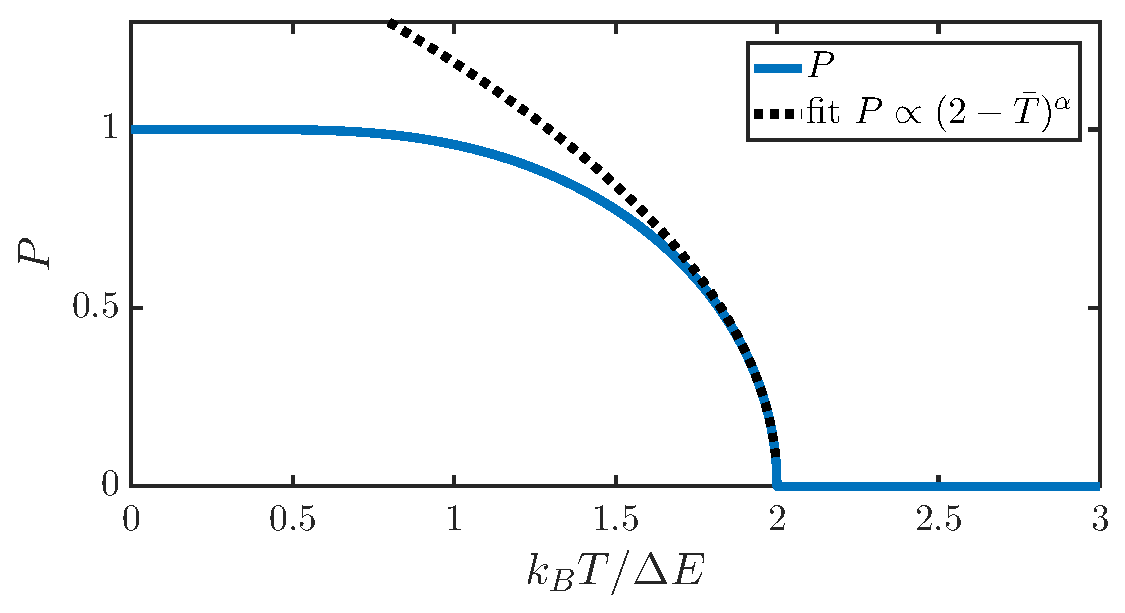
\includegraphics[width=0.7\textwidth]{../figures/P_MFT} 
  \caption{The mean field theory value of the order parameter, $P$, as
  a function of temperature, $\bar{T}=\kB T/\Delta{E}$. There is a
  clear critical temperature, $\bar{T}_{\rm crit}=2$
  ($T_{\rm crit}=\unit[441]{K}$), above which $P$ becomes constantly
  zero. Close below the critical temperature, there is a power law for
  $P(\bar{T})\propto(\bar{T}_{\rm crit}-\bar{T})^{\alpha}$, with
  $\alpha=0.494$; this is shown as the black dotted line. }
  \label{fig:T1:P}
\end{center}
\end{figure}

From the numerical minimization of $F_{\MFT}(P,T)$, we obtained $P(T)$
as shown in figure~\ref{fig:T1:P}. There, we clearly see that there is
a critical temperature at $\bar{T}_{\rm crit}=2$ or, equivalently,
\begin{equation}
T_{\rm crit}=\frac{2\Delta{E}}{\kB}
=\unit[441]{K}=\unit[168]{^{\circ}C}.
\end{equation}
Above this temperature the mean field theory predict that
$P(T>T_{\rm crit})=0$ is constant, which corresponds to a maximally
disordered system. Below the critical temperature $P$ quickly rises to
$P(0)=1$, which is a maximally ordered system. Note, however, that the
sign of $P$ could just as well be flipped since the system is
symmetric under the transformation $P\to-P$ (just switch label on
which sub-lattice is which). There is a symmetry break at $T=T_{\rm
  crit}$, below which the system will spontaneously order itself into
an asymmetric state: $P<0$ or $P>0$.

We can also find an approximating power law near the critical
temperature:
\begin{equation}\label{eq:alpha}
\hat{P}(T)\propto (\bar{T}_{\rm crit}-\bar{T})^{\beta}=(2-\bar{T})^{\beta},
\end{equation}
with a so called \emph{critical exponent}, $\beta$. We used a log-log
fit to find $\beta=0.494$, and the corresponding power relation is
shown as the dotted black line in figure~\ref{fig:T1:P}. 


\begin{figure}[!ht]
\begin{center}
  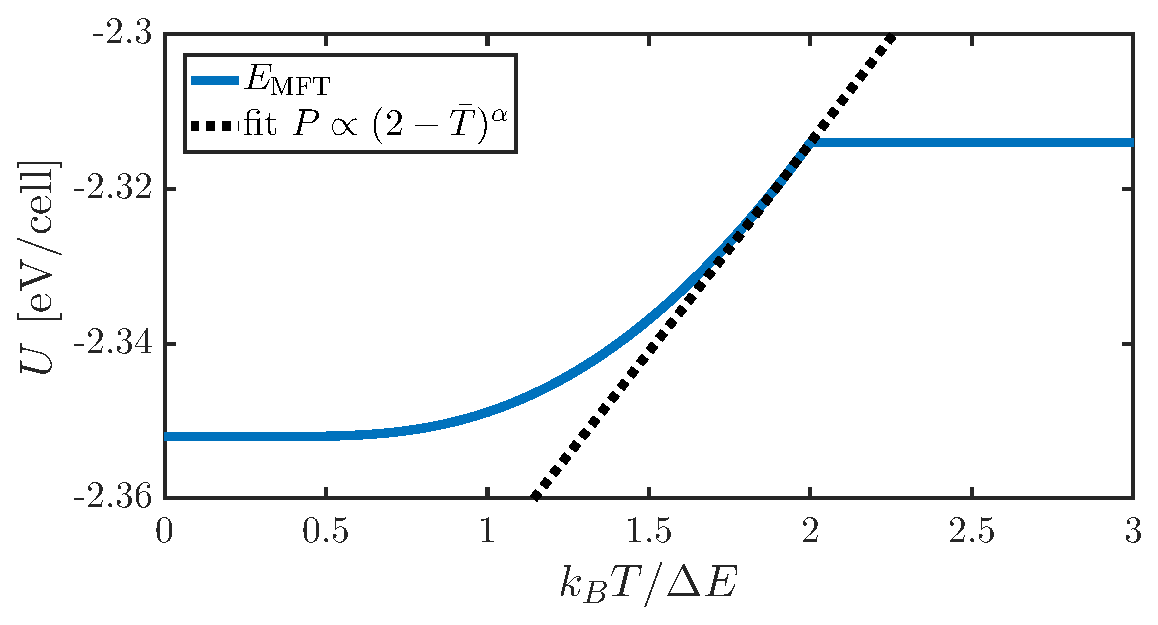
\includegraphics[width=0.7\textwidth]{../figures/E_MFT} 
  \caption{The mean field theory energy per unit cell,
    $u_{\MFT}=U_{\MFT}/N$, as a function of temperature,
    $\bar{T}=\kB T$. The energy rises from
    $u(\bar{T}=0)=E_0-2\Delta{E}=\unit[-2.352]{eV}$ to
    $u(\bar{T}=0)=E_0=\unit[-2.314]{eV}$ per unit cell. }
  \label{fig:T1:E}
\end{center}
\end{figure}

With $P(T)$ found, we can easily use \eqref{eq:E_MFT} to find
$U_{\MFT}(T)=E_{\MFT}(P(T))$, which is plotted in
figure~\ref{fig:T1:E}. There, we see that the energy rises with
temperature, until we reach $\bar{T}=\bar{T}_{\rm crit}=2$ where,
since $P$ becomes constant $P=0$, $U_{\MFT}(T>T_{\rm crit})=N
E_0=-N\times\unit[2.31]{eV}$ becomes constant. We also see that using
the corresponding power law (black dotted line) in $E(\hat{P})$ also
agrees quite well. 

\begin{figure}[!ht]
\begin{center}
  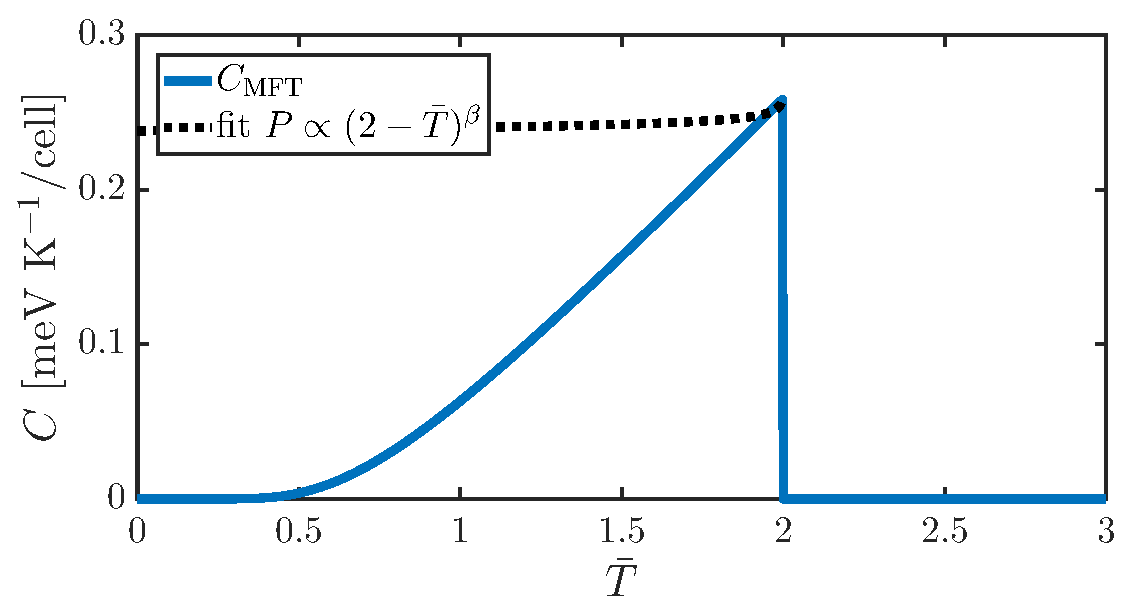
\includegraphics[width=0.7\textwidth]{../figures/C_MFT} 
  \caption{The mean field theory heat capacity, $C_{\MFT}$, as
    function of temperature, $\bar{T}=\kB T/\Delta{E}$. The heat
    capacity rises until $\bar{T}=\bar{T}_{\rm crit}$ to a maximum
    value of about $C_{\MFT}^{(\max)}=\unit[0.26]{meV/K}$ per unit
    cell, above which $C_{\MFT}$ immediately drops to $0$.}
  \label{fig:T1:C}
\end{center}
\end{figure}

Lastly, we can calculate the MFT heat capacity of the system by
numerically differentiate $U$ from before, the result of which is
shown in figure~\ref{fig:T1:C}. Here, we see an almost linear rise in
heat capacity as $T$ approaches $T_{\rm crit}$. Then, above the
critical temperature, the mean field theory heat capacity drops to
$C_{\MFT}(T>T_{\rm crit})=0$. This is clearly not physical since that
would mean that there is no cost in energy to change the temperature
of the system above the critical temperature.

There is also a critical exponent for the heat capacity,
$\hat{C}\propto(\bar{T}_{\rm crit}-\bar{T})^{-\alpha}$. Using
\eqref{eq:C_MFT}, we can easily show that
\begin{equation}
\hat{C}\propto(\bar{T}_{\rm crit}-\bar{T})^{2\beta-1},
\end{equation}
which corresponds to $\alpha=1-2\beta=0.012$. This power law is also
plotted in figure~\ref{fig:T1:C}, but the agreement is much worse than
in the previous two cases.

The first critical exponent we found, $\beta$, is very close to
$1/2$ and it is likely that the value we got deviate from $1/2$
due to numerical errors. If $\beta=1/2$ exactly, then that would
correspond to $\alpha=0$, but that is not really what we see in
figure~\ref{fig:T1:C}.

By now it is clear that the mean field theory model does not provide a
very good representation of the physical system and better methods are
required, such as the numerical simulation in the next task.


%%%%%%%%%%%%%%%%%%%%%%%%%%%%%%%%%%%%%%%%%%%%%%%%%%%%%%%
\section*{Task 2: Ising model}
\begin{align}
E_{\rm CuZn} &= \unit[-294]{meV} \\
E_{\rm CuCu} &= \unit[-436]{meV} \\
E_{\rm ZnZn} &= \unit[-133]{meV} \\
\end{align}

Figure~\ref{fig:T2:equil} shows the equilibration at three different temperatures. We note that the energy per bond is in the range $E_{\rm CuZn} \leq E \leq (E_{\rm CuCu} + E_{\rm ZnZn})/2 = \unit[284.5]{meV}$, which it should be. 

\begin{figure}[!ht]
\begin{center}
  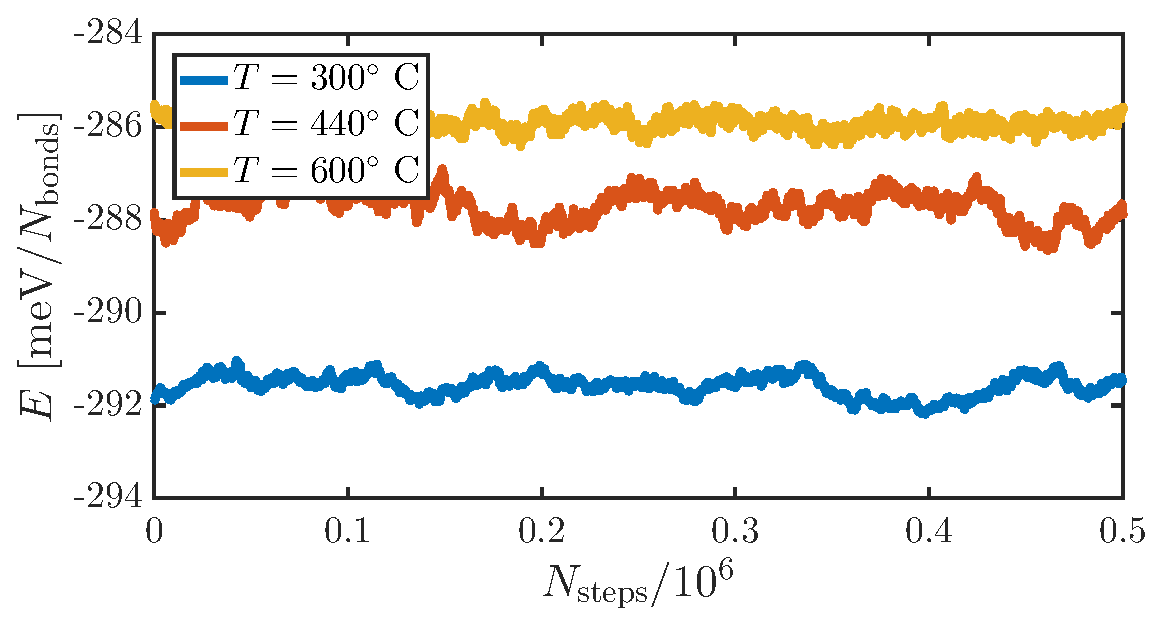
\includegraphics[width=0.7\textwidth]{../figures/equilibration} 
  \caption{... }
  \label{fig:T2:equil}
\end{center}
\end{figure}

\section*{Concluding discussion}
 ...  
\newpage

\appendix

\section{Source Code}

%\subsection{Calculating pi using matlab: \texttt{pi.m}}
%\lstinputlisting[language=matlab,numbers=left]{template_files/pi.m}

%\subsection{Calculating pi using python: \texttt{pi.py}}
%\lstinputlisting[language=python,numbers=left]{template_files/pi.py}

\subsection{Main program task 2: \texttt{main\_T2.c}}
\lstinputlisting[language=c,numbers=left]{../code/main_T2.c}


\subsection{Misc functions : \texttt{funcs.c}}
\lstinputlisting[language=c,numbers=left]{../code/funcs.c}

\section{Auxiliary }
\subsection{Makefile}
\lstinputlisting[language=bash,numbers=left]{../code/Makefile}

\section{MATLAB scripts}
\subsection{Task 1 and analysis scripts for Task 2}
\lstinputlisting[language=matlab,numbers=left]{../m_scripts/H2_analysis.m}

\subsection{Improve figure appearance: \texttt{ImproveFigureCompPhys.m}}
\lstinputlisting[language=matlab,numbers=left]{../m_scripts/ImproveFigureCompPhys.m}

\subsection{Change size of figures: \texttt{setFigureSize.m}}
\lstinputlisting[language=matlab,numbers=left]{../m_scripts/setFigureSize.m}
\end{document}

%%% Local Variables:
%%% mode: latex
%%% TeX-master: t
%%% End:

%  LocalWords:  MFT Helmholz's Ising
